\documentclass{beamer}

\usepackage[utf8]{inputenc}
\usepackage{default}
\usepackage{graphicx}
\usepackage{subfig}
\usepackage{rotating}

\usepackage[]{biblatex}
% \bibliography{refs/refs.bib}

% \pdfminorversion=5

%-----------------------------------------------------%
\renewcommand{\d}{\partial}
%-----------------------------------------------------%

\newcommand{\subfigure}{\subfloat}

\usetheme{Warsaw}
\title[Presentation - Kongsberg Defence \& Aerospace]{Diffusion processes in the brain}
\author{Fredrik E. Pettersen}
\date{\today}



\begin{document}

\begin{frame}
\titlepage
\end{frame}



\begin{frame}
 \frametitle{Contents}
 \tableofcontents[hideallsubsections]
\end{frame}

\section{Introduction}
\begin{frame}
 \frametitle{Brief introduction to the brain}
\end{frame}

\begin{frame}
 \frametitle{Cells in the brain}
 \begin{columns}
\column{2.0in} Neurons:\\
\begin{itemize}
 \item Signal processing
\end{itemize}
% \begin{figure}[H]
%  \centering
%  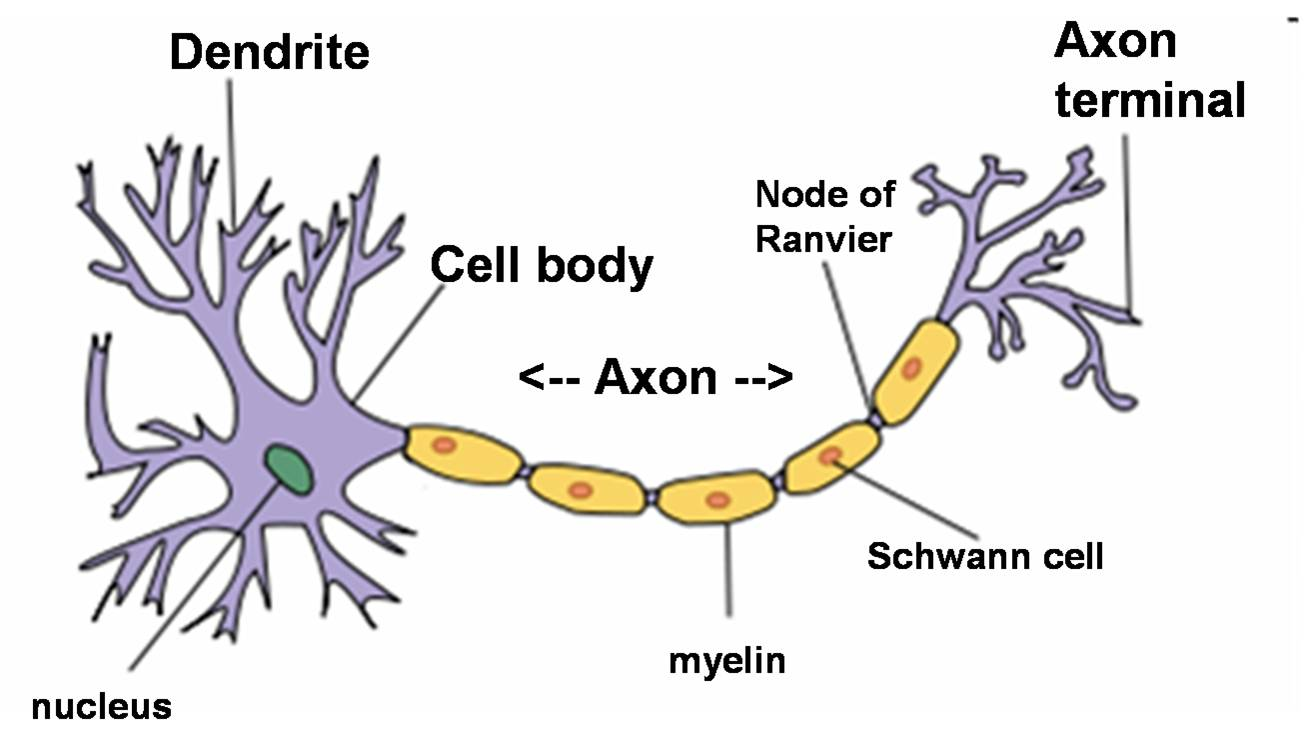
\includegraphics[width=\textwidth]{neuron.jpg}
% \end{figure}

\column{2.0in} Neuroglia:\\
\begin{itemize}
 \item Janitorial tasks
\end{itemize}
% \begin{figure}[H]
%  \centering
%  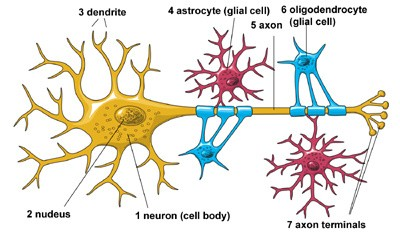
\includegraphics[width=\textwidth]{neuroglia.png}
% \end{figure}
 \end{columns}
\end{frame}


\section{Mathematical models}

\begin{frame}
 \frametitle{Basic diffusion}
 The basic diffusion equation reads
 \begin{equation}
  \frac{\d C}{\d t} = D\nabla^2C
 \end{equation}
Einstein relations
\begin{equation}
 D = \frac{k_B T}{6\pi\eta r}
\end{equation}
\begin{equation}
 \langle r^2\rangle = 2dDt
\end{equation}
\end{frame}



\section{Other possible modeling approaches}
\begin{frame}
 \frametitle{Molecular dynamics}
 \begin{itemize}
  \item Study of systems of atoms and their time-development
  \item Most research towards fracture mechanics and flow in tight rocks
  \item Much of the geometry is similar, but the length scale is a bit to small
  \item Dissipative fluid dynamics
 \end{itemize}
 
\end{frame}

\begin{frame}
 \frametitle{My experiment - motivation}
 \begin{columns}
  \column{2.0in}
  \begin{itemize}
   \item Results from 2003 article by Hrab\v{e}tov\'{a} and Nicholson
   \item Max value of tortuosity $\lambda \leq 1.225$
   \item Diffusion modeling on regular geometries
  \end{itemize}
\column{2.0in}
% \begin{figure}[H]
% \centering
% \includegraphics[width=\textwidth]{octahedra.png}
% \end{figure}

 \end{columns}

\end{frame}

\begin{frame}
 \frametitle{My experiment - results}
 \begin{columns}
  \column{2.0in}
  \begin{itemize}
   \item Making spheres of stationary atoms
   \item Measuring self diffusion constant of liquid using Einstein relation
   \item Comparing to self diffusion constant of bulk fluid
   \item Found $\lambda \approx 1.41$
   \item Limitations
  \end{itemize}
\column{2.0in}
% \begin{figure}[H]
% \centering
% \includegraphics[width=\textwidth]{nanoporous_fluid.png}
%  \end{figure}

 \end{columns}

\end{frame}

\begin{frame}
 \frametitle{Random walks}
 \begin{columns}
  \column{2.0in}
  \begin{itemize}
   \item Percolation theory
   \item Random walks and diffusion
   \item Spanning cluster
   \item Results from by Hrab\v{e}tov\'{a} and Nicholson
   \item Limitations
  \end{itemize}
\column{2.0in}
% \begin{figure}[H]
% \centering
% \includegraphics[width=\textwidth]{oppg_a_percmatrix.png}
%  \end{figure}

 \end{columns}
\end{frame}

\section{Some interesting effects}
\begin{frame}
 \frametitle{Firing in auditory nervous system}
%   \begin{columns}
%   \column{2.0in}
  \begin{itemize}
   \item Unanswered questions 
   \begin{itemize}
    \item limitation of tortuosity
    \item tortuosity constant for increasing $\alpha$
   \end{itemize}
   \item Other modeling methods
   \item Multi scale models; the best from both worlds?
  \end{itemize}
% \column{2.0in}
% \begin{figure}[H]
% \centering
% \includegraphics[width=\textwidth]{oppg_a_percmatrix.png}
%  \end{figure}
% 
%  \end{columns}
\end{frame}

\begin{frame}
\begin{center}
 \textbf{Thank you!}
\end{center}
% \printbibliography
\end{frame}

\begin{frame}
\frametitle{Output from DTI}
% \begin{figure}
%  \includegraphics[scale=0.3]{contest_logo.jpg}
% \end{figure}
\end{frame}

\begin{frame}
\frametitle{Output from DTI}
\end{frame}

\end{document}